\documentclass[a4paper]{article}

%Tutti gli usepackage vanno qui

\usepackage{geometry}
\usepackage[italian]{babel}
\usepackage[utf8]{inputenc}
\usepackage[T1]{fontenc}
\usepackage{tabularx}
\usepackage{longtable}
\usepackage{hyperref}
\usepackage{enumitem}
\hypersetup{
	colorlinks=true,
	linkcolor=black,
	filecolor=magenta,      
	urlcolor=blue,
}
% Numerazione figure 
\let\counterwithout\relax
\let\counterwithin\relax
\usepackage{chngcntr}

\counterwithin{table}{subsection}
\counterwithin{figure}{subsection}

\usepackage[bottom]{footmisc}
\usepackage{fancyhdr}
\usepackage{titlesec}
\setcounter{secnumdepth}{5}
\usepackage{amsmath, amssymb}
\usepackage{array}
\usepackage{graphicx}

%\usepackage{float}
\usepackage{layouts}
\usepackage{url}
\usepackage{comment}
\usepackage{float}
\usepackage{eurosym}


\usepackage{layouts}
\usepackage{float}
\usepackage{eurosym}

%Comandi di impaginazione uguale per tutti i documenti
\pagestyle{fancy}
\lhead{
\includegraphics[scale=0.07]{res/images/zeus_code_logo.png}}
%Titolo del documento
\rhead{\doctitle{}}
%\rfoot{\thepage}
\cfoot{Pagina \thepage\ di \pageref{LastPage}}
\setlength{\headheight}{35pt}
\setcounter{tocdepth}{5}
\setcounter{secnumdepth}{5}
\renewcommand{\footrulewidth}{0.4pt}

% multirow per tabelle
\usepackage{multirow}

% Permette tabelle su più pagine

%\usepackage{longtable}


% colore di sfondo per le celle
\usepackage[table]{xcolor}

%COMANDI TABELLE
\newcommand{\rowcolorhead}{\rowcolor[HTML]{56A5EC}} %intestazione 
\newcommand{\rowcolorlight}{\rowcolor[HTML]{FAFAFA}} %righe chiare/dispari
\newcommand{\rowcolordark}{\rowcolor[HTML]{E1F5FE}} %righe scure/pari
\newcommand{\colorhead}{\color[HTML]{FFFFFF}} %testo intestazione
\newcommand{\colorbody}{\color[HTML]{000000}} %testo righe
\newcommand{\tabitem}{~~\rlap{\textbullet}~~}

\newcommand{\glo}{$_{G}$}
\newcommand{\glosp}{$_{G}$ }

\definecolor{pari}{HTML}{E1F5FE}
\definecolor{dispari}{HTML}{FAFAFA}

%mettere il totale di pagine del doc a piè di pagina
\usepackage{lastpage}
%\fancypagestyle{plain} {
%	\fancyfoot[C]{Pagina \thepage\ di \pageref{LastPage}}}



%Lista dei comandi personalizzati
\newcommand{\doctitle}{Verbale esterno 2019-03-14}
\newcommand{\rev}{1.0.0}
\newcommand{\approv}{Irina Hornoiu}
\newcommand{\ver}{Riccardo Dario}
\newcommand{\red}{Marco Dalla Bà}
\newcommand{\stato}{Approvato}
\newcommand{\uso}{Esterno}
\newcommand{\describedoc}{Riassunto dell'incontro del gruppo \textit{Zeus Code} con GaiaGo tenutosi il 2019-03-11.}
\newcommand{\destinatari}{Zeus Code\\& GaiaGo\\& Prof. Tullio Vardanega\\& Prof. Riccardo Cardin}



\makeindex

\usepackage{hyperref}	%queste due linee le ho aggiunte altrimenti non funzionano i link


\begin{document}
	\thispagestyle{empty}
\begin{titlepage}
	\begin{center}
		
\includegraphics[scale = 0.3]{res/images/zeus_code_logo.png}\\
		\large \textbf{Zeus Code - Progetto "P2PCS"} \\
		\vfill
		\Huge \textbf{\doctitle}
		\vspace*{\fill}
		
		\vfill
		\large
		\begin{tabular}{r|l}
			\textbf{Versione} & \rev{} \\
	%		\textbf{Approvazione} & \approv{} \\
			\textbf{Redazione} & \red{} \\
			\textbf{Verifica} & \ver{} \\
			\textbf{Stato} & \stato{} \\
			\textbf{Uso} & \uso{} \\
			\textbf{Destinato a} & \parbox[t]{5cm}{Zeus Code
				\\Prof. Tullio Vardanega\\Prof. Riccardo Cardin}
		\end{tabular}
		\vfill
		\normalsize
		\textbf{Descrizione}\\
		\describedoc
		\vfill
		\small
		\texttt{zeuscode17@gmail.com}
	\end{center}
\end{titlepage}
	\pagebreak	
	
	\section*{Diario delle modifiche}
\renewcommand{\arraystretch}{1.5}
        \rowcolors{2}{pari}{dispari}
        \begin{longtable}{ 
        		>{\centering}p{0.09\textwidth} 
        		>{\centering}p{0.13\textwidth}
        		>{\centering}p{0.2\textwidth} 
        		>{\centering}p{0.16\textwidth} 
        		>{}p{0.2775\textwidth} }
        	
        	\rowcolorhead
        	\textbf{\color{white}Versione} & 
        	\textbf{\color{white}Data} & 
        	\textbf{\color{white}Nominativo} & 
        	\textbf{\color{white}Ruolo} &
        	\centering \textbf{\color{white}Descrizione} 
        	\tabularnewline  
        	\endfirsthead
        	\rowcolorhead
        	\textbf{\color{white}Versione} & 
        	\textbf{\color{white}Data} & 
        	\textbf{\color{white}Nominativo} & 
        	\textbf{\color{white}Ruolo} &
        	\centering \textbf{\color{white}Descrizione} 
        	\tabularnewline  
        	\endhead
                
                2.0.0 & 2019-04-09 & Andrea Pigatto & \textit{Responsabile di Progetto}
                & Approvazione del documento per RP.\\
                
            	1.1.0 & 2019-05-08 & Marco Dalla Bà & \textit{Verificatore}
            	& Revisione documento.\\
            
            	 1.0.2 & 2019-05-07 & Riccardo Basso & \textit{Analista}
            	& Correzione e inserimento nuovi termini di glossario.\\
            	
            	 1.0.1 & 2019-05-06 & Riccardo Basso & \textit{Analista}
            	& Correzione e inserimento nuovi termini di glossario.\\
            		
            	1.0.0 & 2019-04-09 & Marco Dalla Bà & \textit{Responsabile di Progetto}
            	& Approvazione del documento per RR.\\
            	
                0.2.0 & 2019-04-08 & Diba Meysamiazad & \textit{Verificatore}
                & Revisione intero documento.\\
                
                 0.1.9 & 2019-04-07 & Andrea Pigatto & \textit{Analista}
                & Correzione e inserimento nuovi termini di glossario.\\
                
                 0.1.8 & 2019-04-05 & Irina Hornoiu & \textit{Analista}
                & Correzione e inserimento nuovi termini di glossario.\\
                
                 0.1.7 & 2019-04-04 & Irina Hornoiu & \textit{Analista}
                & Correzione e inserimento nuovi termini di glossario.\\
                
                 0.1.6 & 2019-04-04 & Andrea Pigatto & \textit{Analista}
                & Correzione e inserimento nuovi termini di glossario.\\
                
                0.1.5 & 2019-04-03 & Irina Hornoiu & \textit{Analista}
                & Correzione e inserimento nuovi termini di glossario.\\
                
                0.1.4 & 2019-04-02 & Irina Hornoiu & \textit{Analista}
                & Correzione e inserimento nuovi termini di glossario.\\
                
                0.1.3 & 2019-04-01 & Andrea Pigatto & \textit{Analista}
                & Correzione e inserimento nuovi termini di glossario.\\
                
                0.1.2 & 2019-03-29 & Andrea Pigatto & \textit{Analista}
                & Correzione e inserimento nuovi termini di glossario.\\
                
                0.1.1 & 2019-03-28 & Irina Hornoiu & \textit{Analista}
                & Correzione e inserimento nuovi termini di glossario.\\
                
                0.1.0 & 2019-03-27 & Diba Meysamiazad & \textit{Verificatore}
                & Revisione dei termini inseriti.\\
                
                0.0.9 & 2019-03-26 & Irina Hornoiu & \textit{Analista}
                & Correzione e inserimento nuovi termini di glossario.\\
                
                0.0.8 & 2019-04-25 & Irina Hornoiu & \textit{Analista}
                & Correzione e inserimento nuovi termini di glossario.\\
                
                0.0.7 & 2019-04-23 & Andrea Pigatto & \textit{Analista}
                & Correzione e inserimento nuovi termini di glossario.\\
                
                0.0.6 & 2019-04-22 & Andrea Pigatto & \textit{Analista}
                & Correzione e inserimento nuovi termini di glossario.\\
                
                0.0.5 & 2019-04-21 & Andrea Pigatto & \textit{Analista}
                & Correzione e inserimento nuovi termini di glossario.\\
                
                0.0.4 & 2019-03-21 & Irina Hornoiu & \textit{Analista}
                & Correzione e inserimento nuovi termini di glossario.\\
                
                0.0.3 & 2019-03-20 & Irina Hornoiu & \textit{Analista}
                & Inserimento dei termini di glossario da J a Z manualmente.\\ 
                 
                0.0.2 & 2019-03-20 & Andrea Pigatto & \textit{Analista}
                & Inserimento dei termini di glossario da A a K manualmente.\\

                 
                0.0.1 & 2019-03-19 & Irina Hornoiu & \textit{Analista}
                & Creato documento \LaTeX{} e creata pagina del titolo.\\
                
                 
                
        \end{longtable}


	\pagebreak
	
	\tableofcontents
	
	\pagebreak
	
	\listoffigures
	
	\pagebreak
	
	\pagebreak
	
	\section{Introduzione} 
\subsection{Scopo del documento}
Il presente documento ha lo scopo di analizzare e chiarire i requisiti identificati dal team riguardanti il progetto \textit{P2PCS}. Tali requisiti sono stati identificati dall'analisi del capitolato\glosp C5 e secondo le esigenze del proponente, \textit{GaiaGo}.
\subsection{Scopo del prodotto}
Lo scopo del prodotto è sviluppare un piattaforma di Car Sharing Peer-to-Peer\glosp  per l'applicazione Android sviluppato da GaiaGo per il servizio di Car Sharing Condominiale. L'app mobile verrà sviluppata usando il linguaggio Kotlin\glosp e l'ambiente di sviluppo è Android Studio, mentre per il back end\glosp verrà sfruttato un server AWS\glo. L'obiettivo del capitolato\glosp è quello di realizzare un'app che sfrutti i meccanismi di gamification\glo; a questo fine verrà utilizzato il framework\glosp Octalysis\glo. I servizi scelti dal team per gestire la gamification sono:
\begin{itemize}
	\item {accomplishment};
	\item {ownership};
	\item {unpredictability};
	\item {social influence};
	\item {empowerment}.
\end{itemize}
Il business per \textit{GaiaGo} sarà formato dall'analisi delle abitudini di guida degli utenti e dalla possibilità di vendere altri beni o servizi sulla piattaforma. Perciò lo scopo principale del capitolato commissionato è ridurre al minimo i costi di viaggio, garantendo così un alto utilizzo dell'applicazione. 
A tal scopo si intendono usare i core drive\glosp sopra descritti, ricompensando gli utenti che condividono la propria auto ad un prezzo basso. Il capitolato non richiede la gestione dei pagamenti o altri aspetti come gestione dello scambio di chiavi, l'inserimento della patente, segnalazione dei danni o malfunzionamento dell'auto oppure la gestione dell'aggiornamento dell'app.

\subsection{Glossario}
Con l’obiettivo di evitare ridondanze e ambiguità di linguaggio, i termini tecnici e gli acronimi utilizzati nei documenti verranno definiti e descritti riportandoli nel documento \textit{Glossario v2.0.0}.  I vocaboli riportati vengono indicati con una 'G' a pedice.
\subsection{Riferimenti}
\subsubsection{Normativi}
\begin{itemize}
	\item \textbf{Norme di Progetto}: \textit{Norme di Progetto v2.0.0};

	\item \textbf{Capitolato\glosp d'appalto C5 - P2PCS: piattaforma di Peer-to-Peer\glosp car sharing}: \\ \url{ https://www.math.unipd.it/~tullio/IS-1/2018/Progetto/C5.pdf};
	\item \textbf{Verbale esterno}: \textit{Verbale esterno 2019-03-14};

\end{itemize}
\subsubsection{Informativi}
\begin{itemize}
	\item \textbf{Studio di Fattibilità}: \textit{Studio di Fattibilità v1.0.0};
	\item \textbf{Capitolato\glosp d'appalto C5 - P2PCS: piattaforma di Peer-to-Peer\glosp car sharing}: \\ \url{ https://www.math.unipd.it/~tullio/IS-1/2018/Progetto/C5.pdf};
	\item \textbf{Software Engineering - Ian Sommerville - 10\textsuperscript{th} Edition 2014}
	\subitem - Chapter 4: Requirements engineering;
	\item \textbf{Sito ufficiale del framework\glosp Octalysis\glo}: \\ \textsf{\url{https://www.yukaichou.com/octalysis-tool/}}. 

\end{itemize}
	\pagebreak
	
	\section{Processi primari}
\subsection{Fornitura}
\subsubsection{Scopo}
Lo scopo del processo di fornitura è di determinare le procedure e le risorse necessarie allo svolgimento del progetto. Una volta comprese le richieste del proponente e aver stilato uno \textit{Studio di Fattibilità}, il processo può essere avviato con fine di soddisfare ognuna di queste richieste. Inoltre si deve stipulare e concordare con il proponente un contratto per la consegna del prodotto. Si passa dunque a determinare le procedure, le risorse necessarie, e si sviluppa un \textit{Piano di Progetto} che getterà le basi da perseguire fino alla consegna del materiale prodotto.
	Il processo di fornitura è composto dalle seguenti fasi:
	\begin{itemize}
		\item avvio;
		\item approntamento di risposte alle richieste;
		\item contrattazione;
		\item pianificazione;
		\item esecuzione e controllo;
		\item revisione e valutazione;
		\item consegna e completamento.
	\end{itemize}
	\subsubsection{Aspettative}
	Il gruppo intende mantenere un costante dialogo con il proponente, per avere un riscontro efficace sul lavoro svolto e instaurare un rapporto di collaborazione per quanto riguarda:
	\begin{itemize}
		\item determinare aspetti chiave per far fronte ai bisogni del proponente;
		\item stilare requisiti e vincoli sui processi;
		\item stimare le tempistiche di lavoro;
		\item promuovere una verifica continua;
		\item chiarire eventuali dubbi emersi;
		\item accordarsi sulla qualifica del prodotto.
	\end{itemize}
	\subsubsection{Descrizione}
	Questa sezione tratta le norme che i membri del gruppo \textit{8Lab Solutions} devono rispettare in tutte le fasi di progettazione, sviluppo e consegna del prodotto \textit{Soldino}, al fine di diventare fornitori nei confronti del proponente \textit{Red Babel} e dei committenti Prof. Tullio Vardanega e Prof. Riccardo Cardin.
	\subsubsection{Attività}
		\paragraph{Studio di Fattibilità} \mbox{}\\ \mbox{}\\
		\'E compito del responsabile di progetto organizzare riunioni tra i membri del gruppo al fine di permettere lo scambio di opinioni sui capitolati proposti.
		Lo \textit{Studio di Fattibilità}, redatto dagli analisti, indica per ogni capitolato\glo:
		\begin{itemize}
			\item \textbf{Informazioni generali}: vengono elencate le informazioni di base, come il nome del progetto, il proponente e il committente;
			\item \textbf{Descrizione e finalità del progetto}: viene fatta una presentazione del capitolato\glosp in generale, una descrizione delle caratteristiche principali richieste per il prodotto e viene definito l'obiettivo che si vuole raggiungere;
			\item \textbf{Tecnologie interessate}: viene fatto un elenco delle tecnologie richieste per lo svolgimento, che rientrano nel dominio tecnologico;
			\item \textbf{Aspetti positivi, criticità e fattori di rischio}: vengono esposte le considerazione fatte dal gruppo sugli aspetti positivi e sui fattori di rischio del capitolato\glo;
			\item \textbf{Conclusioni}: vengono esposte le ragioni per la quale il gruppo ha deciso di accettare o scartare il capitolato\glo.
		\end{itemize}
		\paragraph{Piano di Progetto} \mbox{}\\ \mbox{}\\
		Il responsabile, con l'aiuto degli amministratori, redige un \textit{Piano di Progetto} da seguire durante il corso del progetto. Questo documento contiene:
		\begin{itemize}
			\item \textbf{Analisi dei rischi}: vengono analizzati nel dettaglio i rischi che potranno presentarsi e vengono esposte le misure e le modalità attraverso le quali i rischi vengono contenuti o mitigati. Viene anche fornita la probabilità con la quale questi possono presentarsi e il livello di gravità per ciascuno;
			\item \textbf{Modello di sviluppo\glo}: viene descritto il modello di sviluppo\glosp che è stato scelto, indispensabile per la pianificazione;
			\item \textbf{Pianificazione}: vengono pianificate le attività da eseguire nelle diverse fasi del progetto e vengono stabilite le loro scadenze temporali;
			\item \textbf{Preventivo e consuntivo}: viene data una stima di lavoro necessaria per ciascuna fase proponendo così un preventivo per il costo totale del progetto. Viene anche tracciato, un consuntivo di periodo relativo all'andamento rispetto a ciò che è stato preventivato.
		\end{itemize}
		\paragraph{Piano di Qualifica} \mbox{}\\ \mbox{}\\
		I verificatori dovranno redigere un documento, detto \textit{Piano di Qualifica} contenente le strategie da adottare per garantire la qualità del materiale prodotto dal gruppo, e dei processi attuati. Il piano è così suddiviso:
		\begin{itemize}
			\item \textbf{Qualità di processo}: vengono identificati dei processi dagli standard, stabiliti degli obiettivi, escogitate delle strategie per attuarli e individuate le metriche per misurarli e controllarli;
			\item \textbf{Qualità di prodotto}: vengono identificati gli attributi più rilevanti per il prodotto, definiti degli obiettivi per raggiungerli e delle metriche per misurarli;
			\item \textbf{Specifiche dei test}: definiscono una serie di test attraverso i quali il prodotto passa per garantire che soddisfi i requisiti;
			\item \textbf{Standard di qualità}: vengono esposti gli standard di qualità scelti;
			\item \textbf{Valutazioni per il miglioramento:} vengono riportati i problemi e le relative soluzioni nel ricoprire un determinato ruolo e nell'uso degli strumenti scelti;
			\item \textbf{Resoconto delle attività di verifica:} per ogni attività si riportano i risultati delle metriche calcolate in forma di resoconto.
		\end{itemize}
		\subsubsection{Strumenti}
		Di seguito sono elencati gli strumenti utilizzati durante il processo di fornitura.
		\paragraph{Microsoft Excel} \mbox{}\\ \mbox{}\\
		Software della suite Microsoft Office per realizzare fogli elettronici. Usato per fare calcoli, produrre diagrammi, istogrammi e areogrammi, creare tabelle e grafici.
		\paragraph{Microsoft Project} \mbox{}\\ \mbox{}\\
		Per assistere i responsabili di progetto nella pianificazione, nell'assegnazione delle risorse, nella verifica del rispetto dei tempi, nella gestione dei budget e nell'analisi dei carichi di lavoro attraverso la creazioni di diagrammi di Gantt\glo, è stato utilizzato Microsoft Project. \\
		\centerline{\url{https://products.office.com/it-it/project/}}
		%PLACEHOLDER
		\begin{figure}[H]
			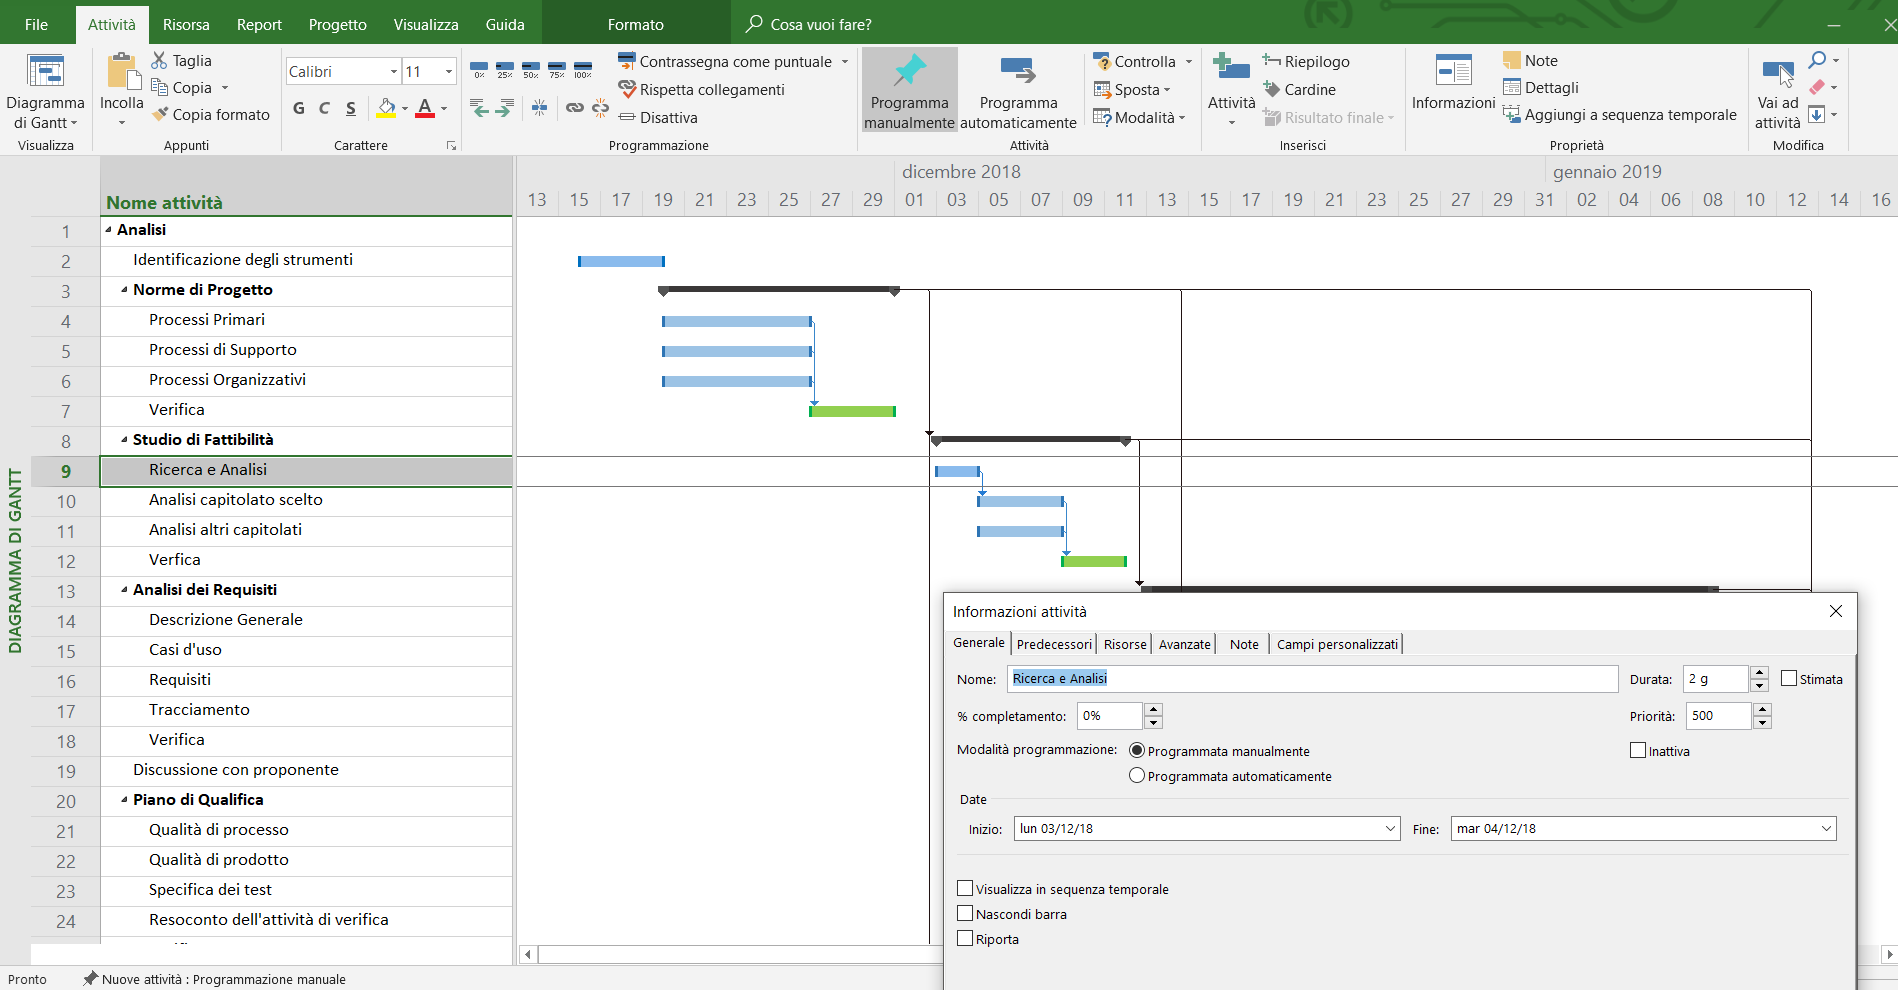
\includegraphics[width=0.99\linewidth]{res/images/projectS.png}
			\caption{Microsoft Project: Gantt}
		\end{figure} 
		\begin{comment}
		\textbf{(questa ultima sezione è da inserire nella fase successiva)}
		\subsubsection{Collaudo e consegna del prodotto}
		Al fine di consegnare il prodotto terminato il gruppo deve effettuare un collaudo in presenza del proponente e dei committenti. Precedentemente a questo test il gruppo deve assicurare correttezza, completezza e affidabilità per ogni parte del materiale consegnato, permettendo così che tutti i requisiti obbligatori siano soddisfatti e l'esecuzione dei test abbiano un esito positivo. In seguito al collaudo finale il responsabile di progetto consegna il prodotto su un supporto fisico.
		\end{comment}
     
\subsection{Sviluppo}
	\subsubsection{Scopo}
	Il processo contiene le attività e i compiti da svolgere, al fine di realizzare il prodotto finale richiesto dal proponente.
	\subsubsection{Aspettative}
	Le aspettative sono le seguenti:
	\begin{itemize}
		\item fissare gli obiettivi di sviluppo;
		\item fissare i vincoli tecnologici;
		\item fissare i vincoli di design;
		\item realizzare un prodotto finale che supera i test, che soddisfa i requisiti e le richieste del proponente.
	\end{itemize}
	\subsubsection{Descrizione}
	Il processo di sviluppo si articola in:
	\begin{itemize}
		\item \textit{Analisi dei Requisiti};
		\item Progettazione;
		\item Codifica.
	\end{itemize}
	\subsubsection{Attività}
		\paragraph{Analisi dei Requisiti} \mbox{}\\ \mbox{}\\
			\textbf{Scopo} \newline \newline
			Gli analisti hanno il compito di redigere il documento di
			\textit{Analisi dei Requisiti} che individua ed elenca dunque, i requisiti.
			Lo scopo dei requisiti è quello di:
			\begin{itemize}
				\item definire lo scopo del lavoro;
				\item fornire ai progettisti riferimenti precisi ed affidabili;
				\item fissare le funzionalità e i requisiti concordati col cliente;
				\item fornire  una  base  per  raffinamenti  successivi  al  fine  di  garantire  un miglioramento continuo del prodotto e del processo di sviluppo;
				\item fornire ai verificatori riferimenti per l'attività di controllo dei test;
				\item calcolare la mole di lavoro per tracciare dei riferimenti per un stima dei costi.
			\end{itemize}
			\textbf{Aspettative} \newline \newline
			Obiettivo dell'attività è la creazione della documentazione formale contenente tutti i
			requisiti richiesti dal proponente. \newline \newline
			\textbf{Descrizione} \newline \newline
			I requisiti si raccolgono secondo modalità predefinite:
			\begin{itemize}
				\item lettura del capitolato\glo, analisi e approfondimento dello stesso;
				\item confronto con il proponente;
				\item confronto tra membri del team di progetto;
				\item analisi di uno o più casi d'uso.  \\
			\end{itemize}
			\noindent
			\textbf{Casi d'uso} \newline \newline
			Rappresenta un diagramma che esprime un comportamento,
			offerto o desiderato, sulla base di risultati osservabili.
			La struttura dei casi d'uso è così suddivisa:
			\begin{itemize}
				\item codice identificativo;
				\item titolo;
				\item diagramma UML\glo;
				\item attori primari;
				\item attori secondari;
				\item descrizione;
				\item scenario principale;
				\item scenario alternativo (se presente);
				\item inclusioni(se presenti);
				\item estensioni(se presenti);
				\item specializzazioni(se presenti);
				\item precondizione;
				\item postcondizione. \\
			\end{itemize}
			\noindent
			\textbf{Codice identificativo dei casi d'uso} \newline \newline
			Il codice di ogni caso d'uso seguirà questo formalismo: \newline \newline
			\centerline{\textbf{UC[codice\_padre].[codice\_figlio]}} \\
			Dove:
			\begin{itemize}
				\item \textbf{codice\_padre}: numero che identifica univocamente i casi d'uso;
				\item \textbf{codice\_figlio}: numero progressivo che identifica i sottocasi. Può a sua volta includere altri livelli. \\
			\end{itemize}
			%\pagebreak
			%esempio di caso d'uso?(immagine)
			\noindent
			\textbf{Requisiti} \newline \newline
			Ogni requisito è composto dalla seguente struttura:
			\begin{itemize}
				\item \textbf{codice identificativo}: ogni codice identificativo è univoco e conforme alla seguente codifica: \\
				\centerline{\textbf{R[Importanza][Tipologia][Codice]}} \\ \\
				Il significato delle cui voci è:
				\begin{itemize}
					\item \textbf{Importanza}: ogni requisito può assumere uno dei seguenti valori:
					\begin{itemize}
						\item \textit{1}: requisito obbligatorio, ovvero irrinunciabile per gli stakeholder;
						\item \textit{2}: requisito desiderabile, ovvero non strettamente necessari ma a valore aggiunto riconoscibile;
						\item \textit{3}: requisito opzionale, ovvero relativamente utile oppure contrattabile più avanti nel progetto;	
					\end{itemize}
					\item \textbf{Tipologia}: ogni requisito può assumere uno dei seguenti valori:
					\begin{itemize}
						\item \textit{F}: funzionale;
						\item \textit{Q}: prestazionale;
						\item \textit{P}: qualitativo;
						\item \textit{V}: vincolo.
					\end{itemize}
					\item \textbf{Codice}: è un identificatore univoco del requisito in forma gerarchica padre/figlio.
				\end{itemize}
				\item \textbf{classificazione}: viene riportata l'importanza del requisito. Sebbene questa sia un'informazione ridondante ne facilita la lettura;
				\item \textbf{descrizione}: descrizione breve ma completa del requisito, meno ambigua possibile;
				\item \textbf{fonti}: ogni requisito può derivare da una o più tra le seguenti opzioni:
				\begin{itemize}
					\item \textit{capitolato\glo}: si tratta di un requisito individuato dalla lettura del capitolato\glo;
					\item \textit{interno}: si tratta di un requisito che gli analisti hanno ritenuto opportuno aggiungere;
					\item \textit{caso d'uso}: il requisito è estrapolato da uno o più casi d'uso. In questo caso deve essere riportato il codice univoco del caso d'uso;
					\item \textit{verbale}: si tratta di un requisito individuato in seguito ad una richiesta di chiarimento con il proponente. Tali informazioni sono riportate nei verbali in cui ogni requisito individuato è segnato da un codice presente nella tabella dei tracciamenti. \\
				\end{itemize}
			\end{itemize}

			\noindent{\textbf{UML}} \newline \newline
			I diagrammi UML\glosp devono essere realizzati usando la versione del linguaggio v2.0.

		\paragraph{Progettazione} \mbox{}\\ \mbox{}\\
			\textbf{Scopo} \newline \newline
			L'attività di progettazione definisce, in funzione dei requisiti specificati nel documento \textit{Analisi dei Requisiti}, le caratteristiche del prodotto software richiesto. Il compito di questa fase è di definire una soluzione del problema che sia soddisfacente per tutti gli stakeholder. La progettazione segue il procedimento inverso rispetto all'\textit{Analisi dei Requisiti} che divide il problema in parti per capirne completamente il dominio applicativo. La progettazione, infatti, rimette insieme le parti specificando le funzionalità dei sottosistemi in modo da ricondurre ad un'unica possibile soluzione. \newline \newline
			\textbf{Aspettative} \newline \newline
			Il processo ha come risultato la realizzazione dell’architettura del sistema. \newline \newline
			\textbf{Descrizione} \newline \newline
			Le parti principali sono due:
			\begin{itemize}
				\item \textbf{Technology baseline}: contiene le specifiche della progettazione ad alto livello del prodotto e delle sue componenti, l'elenco dei diagrammi UML\glosp che saranno utilizzati per la realizzazione dell'architettura e i test di verifica;
				\item \textbf{Product baseline}: dettaglia ulteriormente l'attività di progettazione, integrando ciò che è riportato nella Technology baseline. Inoltre definisce i test necessari alla verifica.
			\end{itemize}
			\textbf{Technology baseline} \newline \newline
			Redatta dal progettista, dovrà includere:
			\begin{itemize}
				\item \textbf{Diagrammi UML\glo}:
				\begin{itemize}
					\item diagrammi delle classi;
					\item diagrammi dei package;
					\item diagrammi di attività;
					\item diagrammi di sequenza.
				\end{itemize}
				\item \textbf{Tecnologie utilizzate}: devono essere descritte le tecnologie adottate specificandone l'utilizzo nel progetto, i vantaggi e gli svantaggi;
				\item \textbf{Design pattern\glo}: devono essere descritti i design pattern\glosp utilizzati per realizzare l'architettura. Ogni design pattern\glosp deve essere accompagnato da una descrizione ed un diagramma, che ne esponga il significato e la struttura;
				\item \textbf{Tracciamento delle componenti}: ogni requisito deve riferirsi al componente che lo soddisfa;
				\item \textbf{Test di integrazione}: l'unione delle parti, intese come classi di verifica, permette di verificare che ogni componente del sistema funzioni nella maniera voluta.
			\end{itemize}
			\textbf{Product baseline} \newline \newline
			A carico del progettista c'è anche la Product baseline che si sofferma su diversi aspetti tra i quali:
			\begin{itemize}
				\item \textbf{definizione delle classi}: ogni classe deve essere descritta in modo da spiegarne in maniera esaustiva lo scopo e le funzionalità, evitando ridondanze;
				\item \textbf{tracciamento delle classi}: ogni requisito deve essere tracciato in modo da garantire che per ognuno esista una classe che lo soddisfi. Questa operazione è fondamentale per permettere di risalire alle classi ad esso associate;
				\item \textbf{test di unità}: devono essere definiti al fine di verificare che le parti funzionino individualmente nel modo stabilito.
			\end{itemize}
		\paragraph{Codifica} \mbox{}\\ \mbox{}\\
			\textbf{Scopo} \newline \newline
			Questa attività ha come scopo quello di normare l'effettiva realizzazione del prodotto software richiesto. In questa fase si concretizza la soluzione attraverso la programmazione. I programmatori dovranno attenersi a queste norme durante la fase di programmazione ed implementazione. \newline \newline
			\textbf{Aspettative} \newline \newline
			Obiettivo dell'attività è la creazione di un prodotto software conforme alle richieste	prefissate con il proponente.
			L'uso di norme e convenzioni in questa fase, è fondamentale per permettere la generazione di codice leggibile ed uniforme,  agevolare le fasi di manutenzione,  verifica e validazione e migliorare la qualità di prodotto. \newline \newline
			\textbf{Descrizione} \newline \newline
			La scrittura del codice dovrà rispettare quanto stabilito nella documentazione di prodotto. Dovrà perseguire gli obiettivi di qualità definiti all'interno del documento \textit{Piano di Qualifica v1.0.0} per poter garantire una buona qualità del codice. \newline \newline
			\textbf{Stile di codifica} \newline \newline
			Al fine di garantire uniformità nel codice del progetto, ciascun membro del gruppo è
			tenuto a rispettare le seguenti norme:
			\begin{itemize}
				\item \textbf{Indentazione}: i blocchi innestati devono essere correttamente indentati, usando per ciascun livello di indentazione quattro (4) spazi (fanno eccezione i commenti). Al fine di assicurare il rispetto di questa regola si consiglia di configurare adeguatamente il proprio editor o IDE;
				\item \textbf{Parentesizzazione}: è richiesto di inserire le parentesi di delimitazione dei costrutti in linea e non al di sotto di essi;
				\item \textbf{Scrittura dei metodi}: è desiderabile, ove possibile, mantenere i metodi brevi(poche righe di codice);
				\item \textbf{Univocità dei nomi}: classi, metodi, variabili devono avere un nome univoco	ed esplicativo al fine di evitare ambiguità e incomprensione;
				\item \textbf{Classi}: i nomi delle classi devono iniziare sempre con una lettera maiuscola;
				\item \textbf{Costanti}: i nomi delle costanti devono essere scritte usando solo maiuscole;
				\item \textbf{Metodi}: i nomi dei metodi devono iniziare con una lettera minuscola. Nel caso
				siano composti da più parole, quelle successive devono iniziare con una lettera maiuscola (CamelCase\glo{});
				\item \textbf{Lingua}: il codice, come anche i commenti, deve essere scritto in lingua inglese.
			\end{itemize}
			Una parte del front end\glosp è normata dalla "Airbnb JavaScript style guide", il cui uso è implementato attraverso ESLint\glo. \newline \newline
			%\subparagraph{Intestazione} \mbox{}\\
			\textbf{Ricorsione} \newline \newline
			L'uso della ricorsione va evitato quanto più possibile in  quanto  potrebbe
			indurre  ad  una  maggiore  occupazione  di  memoria  rispetto  a  soluzioni
			iterative.
	\subsubsection{Strumenti}
	Di seguito sono elencati gli strumenti utilizzati dal gruppo durante il progetto per il processo di sviluppo.
		\paragraph{ESLint} \mbox{}\\ \mbox{}\\
		Utilità open-source per scrivere codice JavaScript secondo regole di codifica predeterminate. Esegue segnalazioni su patterns presenti nel codice ECMAScript/JavaScript.
		\paragraph{PragmaDB} \mbox{}\\ \mbox{}\\
		Programma usato per il tracciamento dei requisiti, fondamentale dunque per la stesura del documento \textit{Analisi dei Requisiti v1.0.0}. \newline
		\centerline{\url{https://github.com/StefanoMunari/PragmaDB}}
		\paragraph{Draw.io} \mbox{}\\ \mbox{}\\
		Per la produzione di diagrammi UML\glosp viene utilizzato Draw.io in quanto offre molte agevolazioni per la produzione veloce dei diagrammi e risulta semplice da usare. \newline
		\centerline{\url{https://www.draw.io/}}
		\begin{figure}[H]
			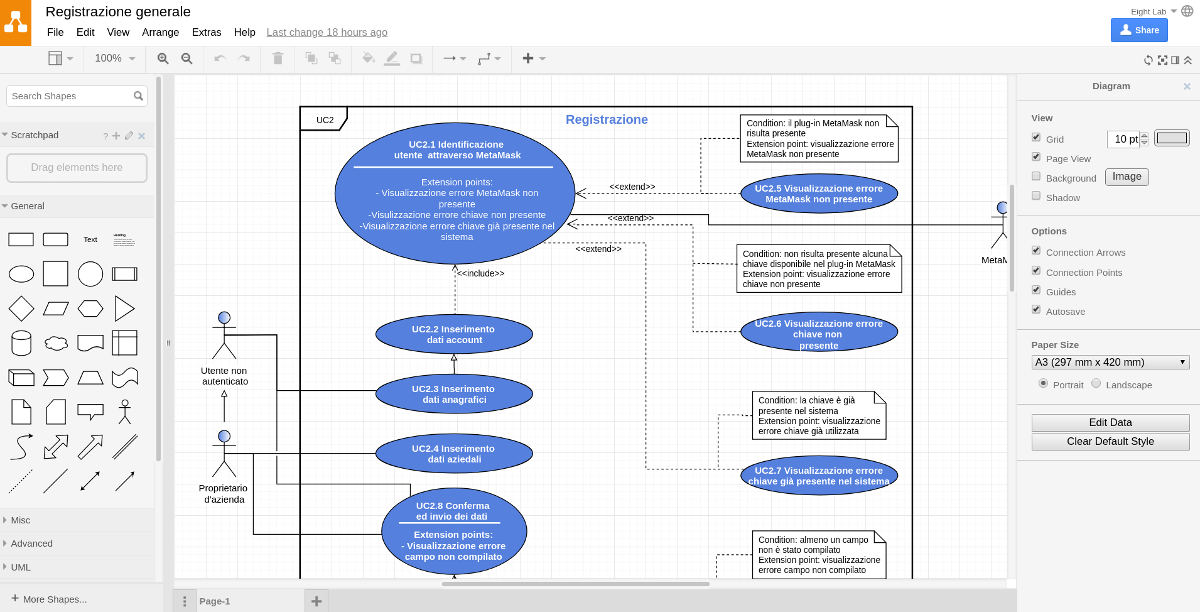
\includegraphics[width=0.99\linewidth]{res/images/drawio.jpg}
			\caption{Software per la creazione di diagrammi online}
		\end{figure} 
		\paragraph{IntelliJ IDEA} \mbox{}\\ \mbox{}\\
		IntelliJ IDEA viene utilizzato per la codifica in Java e JavaScript. Questo IDE offre piena compatibilità con Linux, Windows, macOS, oltre ad essere un potente editor con molte funzionalità integrate. \newline
		\centerline{\url{https://www.jetbrains.com/idea/}}
		\begin{comment}
			\begin{figure}[H]
			\includegraphics[width=0.99\linewidth]{res/images/""}
			\caption{Software per la codifica}
			\end{figure} 
		\end{comment}

	\pagebreak
	
	\section{Processi di supporto}
\subsection{Documentazione}
	\subsubsection{Scopo}
	Ogni processo\glosp e attività significativi volti allo sviluppo del progetto sono documentati. Lo scopo di questa sezione è definire gli standard che riguardano i documenti prodotti durante il ciclo di vita del software.
	I documenti sono consultabili nelle apposite sezioni della repository\glo:\\ \url{https://github.com/ZeusCode17/P2PCS}. 		
	\subsubsection{Aspettative}
	Le aspettative su questo processo riguardano:
	\begin{itemize}
		\item un'idea precisa relativa alla struttura della documentazione che deve essere prodotta durante il ciclo di vita del software;
		\item l'individuazione di una serie di norme per la stesura di documenti coerenti e validi.
	\end{itemize}
	\subsubsection{Descrizione}
	Questo capitolo contiene le decisioni e le norme che sono state scelte per la
	stesura, verifica e approvazione della documentazione ufficiale.  Tali norme  sono  tassative  per  tutti  i  documenti  formali.

	\subsubsection{Template}
	Il gruppo ha creato un template \LaTeX{} per uniformare velocemente la struttura grafica e lo stile di formattazione dei documenti, in modo che i membri del team possano concentrarsi maggiormente, nella stesura del contenuto degli stessi. Lo scopo dei template è quello di permettere, a colui che redige il documento, di adottare automaticamente le conformità previste dalle \textit{Norme di Progetto}. Permette inoltre di agevolare la procedura di adeguamento alle nuove norme per la redazione, nel caso esse cambiassero.
	\subsubsection{Struttura dei documenti}
	Un file "main.tex" (il cui termine "main" verrà sostituito dal nome del documento) raccoglie tramite comandi di input le sezioni di cui è composto il documento. Tra i file in input ci sono:
	\begin{itemize}
		\item "package.tex", che contiene i pacchetti necessari alla compilazione;
		\item "config.tex", contenente comandi \LaTeX{} creati dal team.
	\end{itemize}
		\paragraph{Prima pagina} \mbox{}\\ \mbox{}\\
		Il frontespizio è la prima pagina del documento ed è così strutturata:
		\begin{itemize}
			\item \textbf{Logo del gruppo}: logo di \textit{Zeus Code} visibile come primo elemento centrato orizzontalmente in alto;
			\item \textbf{Gruppo e progetto}: nome del gruppo e del progetto \textit{P2PCS}, visibile centralmente subito sotto il logo;
			\item \textbf{Titolo}: nome del documento, posizionato centralmente in grassetto;
			\item \textbf{Tabella}: presente sotto il titolo del documento, centrale e contenente le seguenti informazioni:
			\begin{itemize}
				\item \textbf{Versione}: versione del documento;
				\item \textbf{Approvazione}: nome e cognome dei membri del gruppo incaricati dell'approvazione del documento;
				\item \textbf{Redazione}: nome e cognome dei membri del gruppo incaricati della redazione del documento;
				\item \textbf{Verifica}: nome e cognome dei membri del gruppo incaricati della verifica del documento;
				\item \textbf{Stato}: stadio corrente del ciclo di vita del documento;
				\item \textbf{Uso}: tipo d'uso che può essere "interno" o "esterno";
				\item \textbf{Destinato a}: destinatari del documento.
			\end{itemize}
			\item \textbf{Descrizione}: descrizione sintetica relativa al documento, centrale, posta sotto la tabella descrittiva;
			\item \textbf{Recapito}: indirizzo di posta elettronica del gruppo, posizionato centralmente in fondo alla pagina.
		\end{itemize}
		\paragraph{Registro delle modifiche} \mbox{}\\ \mbox{}\\
		Ogni documento dispone di un changelog\glo: una tabella posta a seguito della prima pagina che contiene le modifiche apportate al documento. Nel changelog sono indicati:
		\begin{itemize}
			\item versione del documento dopo la modifica;
			\item data della modifica;
			\item nominativo di chi ha modificato;
			\item ruolo di chi ha modificato;
			\item descrizione sintetica della modifica.
		\end{itemize}
		\paragraph{Indice} \mbox{}\\ \mbox{}\\
		Gli indici hanno lo scopo di riepilogare e dare una visione macroscopica della struttura del documento, mostrando le parti gerarchiche di cui è composto.\newline 
		Ogni documento è corredato dall'indice dei contenuti, posizionato dopo il changelog\glo. Se sono presenti tabelle o immagini all'interno del documento, l'indice dei contenuti è seguito prima dalla lista delle figure, poi dalla lista delle tabelle.
		\paragraph{Contenuto principale} \mbox{}\\ \mbox{}\\
		La struttura delle pagine di contenuto è così strutturata:
		\begin{itemize}
			\item in alto a sinistra è presente il logo del gruppo;
			\item in alto a destra è riportato il nome del documento;
			\item una riga divide l'intestazione dal contenuto;
			\item il contenuto della pagina è posto tra l'intestazione e il piè pagina;
			\item una riga divide il contenuto dal piè pagina;
			\item in basso è posto il numero della pagina corrente ed il numero di pagine totali.
		\end{itemize}
		\paragraph{Verbali} \mbox{}\\ \mbox{}\\
		I verbali vengono prodotti dal/i soggetto/i incaricato/i alla loro stesura in occasione di incontri tra i membri del team con o senza la presenza di esterni. Per i verbali è prevista un'unica stesura. Tale	scelta è motivata dal fatto che apportare modifiche implica una modifica delle decisioni prese in modo retroattivo.
		I verbali seguono la struttura degli altri documenti, ma il corpo del verbale è suddiviso in introduzione e contenuto.
		L'introduzione contiene:
		\begin{itemize}
			\item \textbf{Luogo}: luogo di svolgimento dell'incontro;
			\item \textbf{Data}: data dell'incontro(in formato YYYY-MM-DD);
			\item \textbf{Ora di inizio}: l'orario di inizio dell'incontro;
			\item \textbf{Ora di fine}: l'orario di fine dell'incontro;
			\item \textbf{Partecipanti}: l'elenco dei membri del gruppo che erano presenti all'incontro e, se presenti, i nominativi di persone esterne al gruppo che hanno partecipato. Un esempio, sono i nomi dei componenti di \textit{GaiaGo}, a fianco al quale deve essere indicato "(proponente)";
			\item \textbf{Argomenti affrontati}: ciò di cui si è discusso durante l'incontro in forma riassuntiva e facendo risaltare gli argomenti principali.
		\end{itemize}
	Il contenuto è composto da:
	\begin{itemize}
		\item una descrizione più approfondita in merito agli argomenti trattati durante l'incontro sotto forma di elenco puntato. Tale elenco riporta gli eventi nell'ordine in cui sono avvenuti;
		\begin{itemize}
			\item ogni voce dell'elenco principale dei contenuti deve comincia per lettera \textbf{maiuscola}, mentre i sotto-elenchi devono rispettare le norme degli elenchi puntati riportati in seguito;
		\end{itemize}
		
		\item un riepilogo dei tracciamenti in forma tabellare che elenca le decisioni emerse: assegna ad ognuna di loro un codice e le descrive. Sarà ripresa successivamente.
		
	\end{itemize}
		Ogni \textit{Verbale} dovrà essere denominato secondo il seguente formato: \newline \newline
		\centerline{\textbf{TipologiaYYYY-MM-DD}} \newline \newline
		dove per "Tipologia" si intende il tipo di verbale:
		\begin{itemize}
			\item \textbf{Interno}: concentrato sul riassunto dell'incontro dei membri del team;
			\item \textbf{Esterno}: concentrato sulla trattazione di argomenti con partecipanti esterni al gruppo, in particolare domande e risposte riguardanti il progetto in sé.
		\end{itemize}
		La sezione "Riepilogo tracciamenti" avrà la funzione di tenere traccia delle decisioni emerse da ogni incontro, sotto forma di tabella riassuntiva a fine di ogni verbale. Il formalismo utilizzato dalla tabella dovrà essere il seguente: \newline \newline
		\centerline{\textbf{Tipologia\_X.Y}} \newline \newline
		Dove:
		\begin{itemize}
			\item per "Tipologia" basterà indicare l'iniziale della tipologia del verbale(I=Interno/E=Esterno);
			\item "X.Y": X si riferisce al numero dell'incontro mentre per Y si intende il numero progressivo della decisione presa dal gruppo(partendo da 1).
		\end{itemize}	
		\paragraph{Note a piè di pagina} \mbox{}\\ \mbox{}\\
		In caso di presenza di note da esplicare, esse vanno indicate nella pagina corrente, in basso a sinistra. Ogni nota deve riportare un numero e una descrizione.		
	\subsubsection{Norme tipografiche}
		\paragraph{Convenzioni sui nomi dei file} \mbox{}\\ \mbox{}\\
		I nomi di file (estensione esclusa) e cartelle utilizzano la convenzione "Snake case\glo" e alcune regole aggiuntive elencate di seguito:
		\begin{enumerate}
			\item i nomi dei file composti da più parole usano il carattere underscore come carattere separatore;
			\item i nomi sono scritti interamente in minuscolo;
			\item le preposizioni non si omettono.
		\end{enumerate}
		Alcuni esempi \textbf{corretti} sono:
		\begin{itemize}
			\item studio\_di\_fattibilità;
			\item analisi\_dei\_requisiti.
		\end{itemize}	 	
		Alcuni esempi \textbf{non corretti} sono: 
		\begin{itemize}
			\item Norme\_di\_progetto (usa maiuscole);
			\item norme-di-progetto (carattere separatore errato);
			\item norme\_progetto (omette "di").
		\end{itemize}
		\paragraph{Glossario}
		\begin{itemize}
			\item ogni termine del Glossario è marcato con una \textbf{G} maiuscola a pedice in ogni sua occorrenza;
			\item se la voce è presente ripetutamente nello stesso paragrafo non è necessario marcarla in ogni sua occorrenza, ma è possibile indicare la \textbf{G} a pedice solo nella prima occorrenza;
			\item se nel \textit{Glossario v2.0.0} un termine presenta una descrizione che utilizza termini da glossario, è necessario trattare questi termini come tali, segnando la \textbf{G} a pedice e aggiungendoli al documento con la relativa descrizione;
			\item non vengono segnate con la \textbf{G} a pedice  le parole da \textit{Glossario} presenti nei titoli e nelle didascalie di immagini e tabelle.
		\end{itemize}			
		\paragraph{Stile del testo}
		\begin{itemize}
			\item \textbf{Grassetto}:
			viene applicato se necessario alle voci di un elenco puntato, a titoli o a termini di frasi su cui si vuol far ricadere l'attenzione del lettore;
			\item \textbf{Corsivo}: vengono scritti in corsivo il nome del progetto \textit{P2PCS}, il nome del gruppo \textit{Zeus Code}, il nome del gruppo dei proponenti, ovvero \textit{GaiaGo} e nomi dei ruoli all'interno del progetto (es. \textit{Analista}, \textit{Verificatore}); %token\glosp coniato nella piattaforma,  \textit{Cubit};
			\item \textbf{Maiuscolo}: vengono scritti con sole lettere maiuscole tutti gli acronimi. Nel caso di nomi o titoli composti da più parole verrà indicato con la lettera maiuscola solamente la prima lettera della prima parola, lasciando in minuscolo il restante (esclusi nomi dei documenti che sono normati secondo quanto segue);
			\item \textbf{Nomi dei documenti}:
			\begin{itemize}
				\item ogni volta che si cita un documento, si deve indicare con la lettera maiuscola le iniziali dei nomi di cui è composto (\textit{e.g.} Analisi dei Requisiti), ma senza specificare la versione, riportando il tutto in corsivo;
				\item quando si fa riferimento al documento vero e proprio o a qualcosa in esso contenuto si segue la prima convenzione ma si aggiunge la versione del documento v*.0.0 (separata da uno spazio), anch'essa in corsivo;
				\item ogni volta che si utilizza il documento come titolo o in una voce di elenco seguita da una descrizione, si deve seguire la prima convenzione ma senza utilizzare il corsivo.
			\end{itemize}
		\end{itemize}
		\paragraph{Elenchi puntati} \mbox{}\\ \mbox{}\\
		Ogni voce di un elenco comincia per lettera \textbf{minuscola}, a patto che non subentrino altre norme, e termina per \textbf{";"}, eccetto l'ultima che termina per \textbf{"."}. I sotto-elenchi innestati dentro una voce di elenco, rispettano le medesime regole, poiché la loro funzione è analoga.\newline
		Se le voci dell'elenco sono della forma \textit{termine - descrizione}, si pongono i termini in grassetto.
		\paragraph{Formati comuni} \mbox{}\\ \mbox{}\\
		In conformità allo standard ISO 8601, le date devono essere scritte secondo il formato: \newline \newline
		\centerline{YYYY-MM-DD}
		\begin{itemize}
			\item \textbf{YYYY}: rappresentazione dell'anno con quattro (4) cifre;
			\item\textbf{MM}: rappresentazione del mese con due (2) cifre;
			\item \textbf{DD}: rappresentazione del giorno con due (2) cifre.			
		\end{itemize}
		\paragraph{Sigle} \mbox{}\\ \mbox{}\\
		Il progetto prevede la redazione di un insieme di documenti, suddivisi in documenti interni\glosp e documenti esterni\glo. Essi sono elencati di seguito con le rispettive sigle.\newline
		I documenti esterni sono:	
		\begin{itemize}
			\item \textbf{Analisi dei Requisiti - AdR}: stabilisce le caratteristiche che il software deve rispettare;
			\item \textbf{Manuale Utente - MU}: ad uso degli utilizzatori del software;
			\item \textbf{Manuale Sviluppatore - MS}: per gli sviluppatori e manutentori;
			\item \textbf{Piano di Progetto - PdP}:  concerne la gestione del progetto, evidenziandone la fattibilità e le criticità; tratta di tempi, costi, obiettivi, rischi, vincoli;
			\item \textbf{Piano di Qualifica - PdQ}: : descrive la qualità del software e dei processi, e come la si intende raggiungere mediante l'uso di strumenti, metriche e processi stessi;
			\item \textbf{Glossario - G}: raccoglie i termini di interesse per il team di sviluppo e sui quali è necessaria una descrizione che ne chiarisca il significato.
		\end{itemize}
		I documenti interni sono:
		\begin{itemize}
			
			\item \textbf{Norme di Progetto - NdP}: sono un riferimento normativo per lo svolgimento delle attività di progetto;
			\item \textbf{Studio di Fattibilità - SdF}: descrive sommariamente i capitolati e spiega la loro scelta o esclusione.
		\end{itemize}
		Un caso particolare di documenti, sono i verbali, che possono essere esterni o interni:
		\begin{itemize}
			\item \textbf{Verbale - V}: descrive le interazioni avvenute durante un incontro con il proponente (verbale esterno) o tra i membri del team (verbale interno); sono orientati a dare informazioni semplici, di veloce lettura e complete.
		\end{itemize}
		Le diverse fasi del progetto sono le seguenti, accompagnate dalle relative sigle:
		\begin{itemize}
			\item \textbf{Revisione dei Requisiti - RR}: studio iniziale del capitolato\glo, se ben fatto permette al gruppo di aggiudicarselo;
			\item \textbf{Revisione di Progettazione - RP}: riguarda la definizione dell'architettura del software e di una Proof of Concept\glosp per mostrare la fattibilità;
			\item \textbf{Revisione di Qualifica - RQ}: riguarda la definizione dettagliata e la codifica del prodotto;
			\item \textbf{Revisione di Accettazione - RA}: se il prodotto soddisfa i requisiti del proponente, viene accettato e rilasciato.		
		\end{itemize}	
		Altre sigle presenti nei documenti interessano i ruoli assunti dai componenti del team:
		\begin{itemize}
			\item \textbf{responsabile di progetto - Re};
			\item \textbf{amministratore - Ad};
			\item \textbf{analista - An};
			\item \textbf{progettista - Pt};
			\item \textbf{programmatore - Pr};
			\item \textbf{verificatore - Ve};
		\end{itemize}
		\subsubsection{Elementi grafici}
		\paragraph{Tabelle} \mbox{}\\ \mbox{}\\
		In tutti i documenti \LaTeX{} le tabelle sono scritte allo stesso modo: fare riferimento alla Wiki su GitHub\glosp per i comandi necessari.\newline 
		Ogni tabella deve essere accompagnata dalla propria didascalia descrittiva, la "caption", da posizionare subito sopra la tabella a cui si riferisce. \'E stata scelta questa convenzione per adattarsi agli standard usati dalla maggioranza della community di \LaTeX{}; nella didascalia deve comparire il numero della sezione a cui si riferisce, seguita in modo incrementale dal numero progressivo delle tabelle di quella sezione.
		\begin{itemize}
			\item \textbf{{X.Y}}: rappresenta la sezione;
			\item \textbf{{Z}}: rappresenta il numero progressivo della tabella nella sezione.
		\end{itemize}
		Fanno eccezione le tabelle dei changelog\glosp che non hanno didascalia e le tabelle dei casi d'uso presenti nel documento \textit{Analisi dei Requisiti}.
		\paragraph{Immagini} \mbox{}\\ \mbox{}\\
		Le immagini sono centrate e hanno una didascalia descrittiva. 
		\paragraph{Diagrammi UML} \mbox{}\\ \mbox{}\\
		Tutti i diagrammi UML\glosp vengono inseriti nei documenti sotto forma di immagine.
	\subsubsection{Strumenti}
		\paragraph{\LaTeX} \mbox{}\\ \mbox{}\\
		Lo strumento scelto per la scrittura di documenti è \LaTeX{}, un linguaggio basato sul programma di composizione tipografica \TeX{} che permette di scrivere documenti in modo ordinato, modulare, collaborativo e scalabile.
		\paragraph{\TeX{}studio} \mbox{}\\ \mbox{}\\
		Per la stesura del codice \LaTeX{} è stato utilizzato l'editor \TeX{}studio. Questo strumento, oltre ad integrare un compilatore e un visualizzatore PDF, fornisce suggerimenti di completamento per comandi \LaTeX{}. \newline
		\centerline{\url{https://www.texstudio.org/}}
		\begin{figure}[H]
			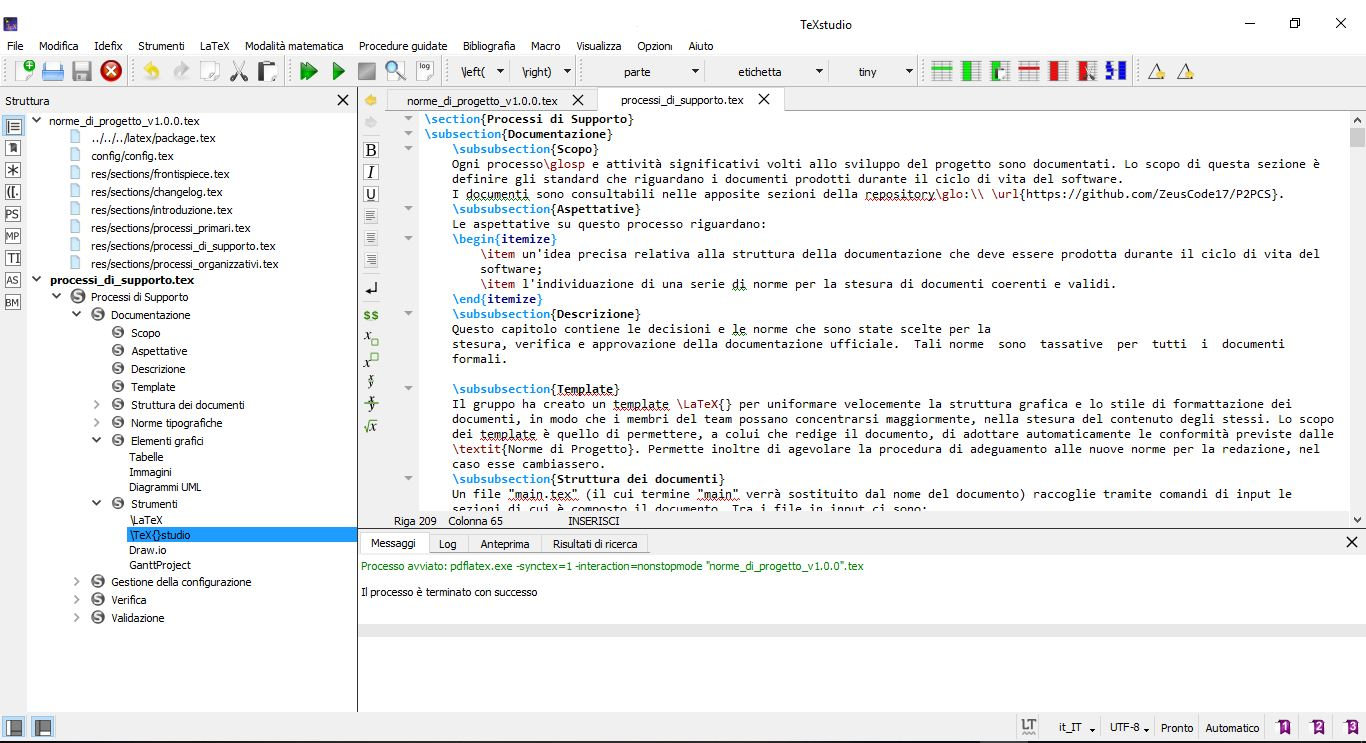
\includegraphics[width=1\linewidth]{res/images/latex2.jpg}
			\caption{\TeX{}studio - per la stesura dei documenti}
		\end{figure} 
		\paragraph{Draw.io} \mbox{}\\ \mbox{}\\
		Draw.io, già citato in precedenza, viene utilizzato per la produzione degli UML\glo. \newline
		\centerline{\url{https://www.draw.io/}}
		
		\paragraph{GanttProject} \mbox{}\\ \mbox{}\\
		GanttProject viene utilizzato per la costruzione dei diagrammi				di Gantt\glo. \newline
		\centerline{\url{https://www.ganttproject.biz/}}
		\begin{figure}[H]
			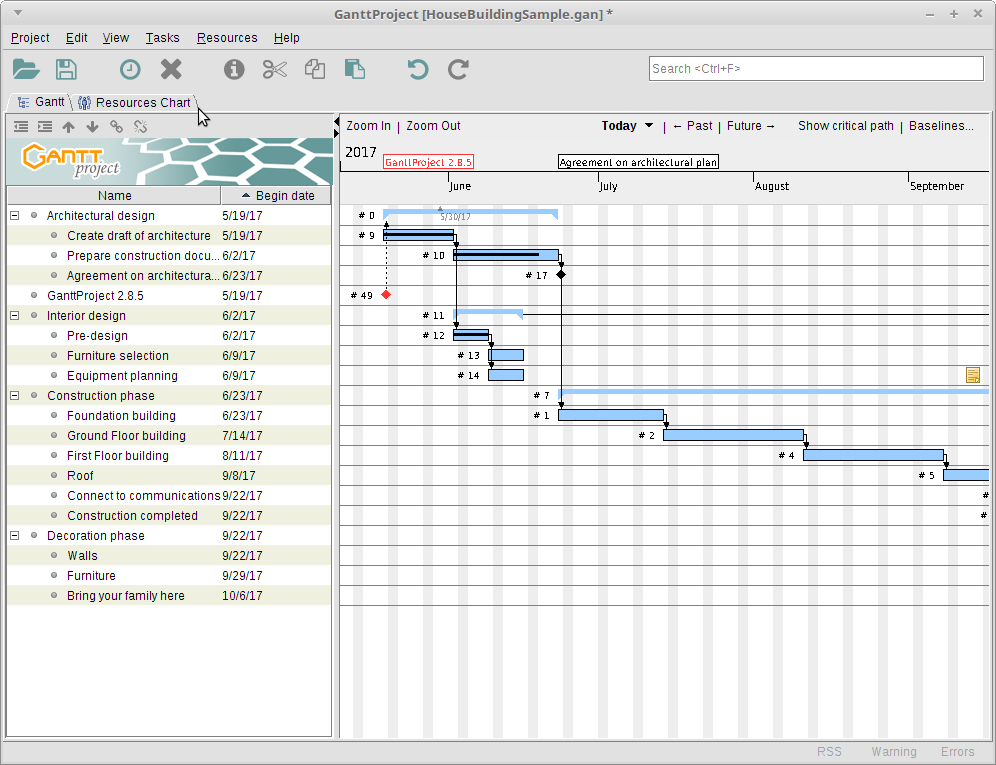
\includegraphics[width=0.99\linewidth]{res/images/ganttproj.png}
			\caption{GanttProject - creazione diagrammi di Gantt}
		\end{figure} 
		
	\subsection{Gestione della configurazione}
	\subsubsection{Scopo}
	Lo scopo ultimo della configurazione è di creare coesione tra software e documenti. Ogni file è caratterizzato da un identificativo univoco, si trova in uno stato di versionamento ed è modificato secondo determinate procedure.
	\subsubsection{Ciclo di vita della documentazione}
	\paragraph{Stadi del documento} \mbox{}\\ \mbox{}\\
	Ogni documento deve necessariamente passare per i seguenti stadi:
	\begin{itemize}
		\item \textbf{Sviluppo}: il documento entra in questo stato da quando viene creato fino al momento della verifica. In questo stato il documento viene redatto e sviluppato in ogni sua parte da un Redattore.
		\item \textbf{Verifica}: il documento entra in questo stato dopo la sua stesura fino al momento dell'approvazione. In questo stato il documento viene controllato in ogni sua parte e in caso di esito positivo passa alla fase di approvazione, in caso contrario verrà riassegnato ad un Redattore per apportare le eventuali migliorie o aggiunte.
		\item \textbf{Approvazione}: il documento entra in questo stato dopo la sua approvazione da parte di un Verificatore. In questo stato il documento viene approvato dal Responsabile del progetto a seguito del superamento della parte di verifica.
	\end{itemize}
	\subsubsection{Versionamento}
	\paragraph{Codice di versione del documento} \mbox{}\\ \mbox{}\\
	Ogni documento è sottoposto a versionamento, ciò permette ai membri del gruppo, o ad utenti esterni, di risalire all'insieme delle modifiche effettuate su quest'ultimo. Ogni versione è riportata nel registro delle modifiche presente ad inizio documento.
	Il numero di versione è composto da tre cifre:
	\begin{center}
		X.Y.Z
	\end{center}
	\begin{itemize}
		\item \textbf{X}: versione ufficiale del documento resa tale dopo l' approvazione da parte del Responsabile di progetto:
		\begin{itemize}
			\item inizia da 0;
			\item viene incrementato dal responsabile di progetto all'approvazione del documento.
		\end{itemize}
		\item \textbf{Y}: versione del documento soggetta a verifica da parte di un Verificatore:
		\begin{itemize}
			\item inizia da 0;
			\item viene incrementato dal Verificatore ad ogni verifica;
			\item quando viene incrementato X, viene riportato a 0.
		\end{itemize}
		\item \textbf{Z}: versione del documento in fase di lavorazione da parte dei Redattori:
		\begin{itemize}
			\item inizia da 0;
			\item viene incrementato dal redattore del documento ad ogni modifica;
			\item quando viene incrementato Y, viene riportato a 0.
		\end{itemize}			
	\end{itemize}
	\paragraph{Tecnologie} \mbox{}\\ \mbox{}\\
	E' stato scelto il sistema Git per il versionamento dei file di progetto, la repository\glosp remota è invece ospitata dal servizio GitHub\glo. 
	\paragraph{Repository} \mbox{}\\ \mbox{}\\
	L'accesso alla repository\glosp da parte dei membri del gruppo è possibile tramite linea di comando o con l'uso di software come GitHub Desktop e simili.
	La versione ufficiale ed aggiornata della repository la si trova al seguente indirizzo di GitHub\glo. \newline \newline
	\centerline{\url{https://github.com/ZeusCode17/P2PCS}}
	\paragraph{Struttura del repository} \mbox{}\\ \mbox{}\\
	Sono presenti due tipi di repository\glosp con uguale struttura:
	\begin{itemize}
		\item \textbf{locale}: repository locale clonata sul pc di ogni membro del gruppo nella quale vengono eseguite le modifiche.
		\item \textbf{remoto}: repository remota ospitata su GitHub\glosp aggiornata con tutte le modifiche apportate da ogni membro del gruppo.
	\end{itemize}			
	Entrambi i tipi di repository sono organizzati in cartelle:
	\begin{itemize}
		\item \textbf{latex}: contiene tutti i file che definiscono il template \LaTeX{} per la creazione di un nuovo documento. Tra questi vi sono i file che definiscono i comandi personalizzati utilizzati dal gruppo e i package che devono essere inclusi per poter compilare i documenti;
		\item \textbf{RR}: raccoglie i file sorgenti per la compilazione dei documenti, suddivisi tra esterni ed interni, realizzati per la Revisione dei Requisiti;
		\item Saranno aggiunte in futuro cartelle distinte nominate \textbf{RP}, \textbf{RQ} e \textbf{RA} contenenti i file delle rispettive consegne.
	\end{itemize}
	Abbiamo scelto la suddivisione dei file per revisione, ciò evidenzia in modo chiaro il lavoro svolto prima di ogni consegna e rende efficacie la tracciabilità dei file.
	\paragraph{Tipi di file e .gitignore} \mbox{}\\ \mbox{}\\
	I file utilizzati per la documentazione del progetto sono:
	\begin{itemize}
		\item file con estensione .tex di \LaTeX{}, contenenti il codice sorgente del file;
		\item file con estensione .pdf che sono oggetto di consegna;
		\item file testuali e immagini impiegati nei file \LaTeX{} e .pdf.
	\end{itemize}			
	Il file ".gitignore" è presente al livello più esterno della repository\glosp ed elenca tutti i file da escludere dal versionamento. 
	\paragraph{Utilizzo di Git} \mbox{}\\ \mbox{}\\
	Il repository\glosp di Git è composto da diversi branch, ciò permette di lavorare in modo parallelo tra i membri del team.  
	I passaggi che vengono eseguiti sono i seguenti:
	\begin{itemize}
		\item viene scelto il branch su cui si intende lavorare;
		\item si esegue il pull dal repository remoto che effettua l'aggiornamento del proprio repository locale;
		\item si svolge il lavoro assegnato,che varia dalla modifica all'aggiunta di nuovi file;
		\item si aggiungono i nuovi file o file modificati all'area di staging\glosp prima di eseguire il commit;
		\item si esegue il comando di commit dei file aggiunti, con annesso un messaggio che identifica il lavoro effettuato;
		\item si esegue il push del commit sul repository remoto.
	\end{itemize}
	\paragraph{Gestione delle modifiche} \mbox{}\\ \mbox{}\\
	Per effettuare semplici modifiche quali errori grammaticali o migliorie di lessico non è necessaria alcuna approvazione dal responsabile del progetto, è necessario però allegare al commit un messaggio chiaro che indica le modifiche effettuate.
	Per quanto riguarda modifiche maggiori la procedura da seguire è la seguente:
	\begin{itemize}
		\item contattare il responsabile del file da modificare;
		\item suggerire la modifica da effettuare;
		\item se il responsabile valuta positivamente la modifica, allora la applica o da il permesso di modifica.
	\end{itemize}
		
\subsection{Verifica}
	Lo scopo del processo di verifica è la realizzazione di prodotti corretti, coesi e completi. La verifica viene effettuata sia sul software che sui documenti. 
	\subsubsection{Aspettative}
	Il processo di verifica rispetta i punti seguenti:	
	\begin{itemize}
		\item effettuato seguendo procedure definite;
		\item criteri chiari e affidabili da seguire per verificare il prodotto;
		\item ogni fase successiva attraversata dal prodotto è verificata;
		\item la verifica porta il prodotto in uno stato stabile;
		\item rende possibile la validazione.
	\end{itemize}
	\subsubsection{Descrizione}
	Il processo di verifica prende in input ciò che è già stato prodotto e lo restituisce in uno stato conforme alle aspettative. Per ottenere tale risultato ci si affida a processi di analisi e test.
	\subsubsection{Attività}
		\paragraph{Analisi} \mbox{}\\ \mbox{}\\
		Il processo di analisi consiste nell'analisi del codice sorgente e nella sua successiva esecuzione. Si suddivide in statica e dinamica.\\
			\subparagraph{Analisi statica} \mbox{}\\ \mbox{}\\
			L'analisi statica effettua controlli su documenti e codice, di cui valuta e applica la correttezza (intesa come assenza di errori e difetti), la conformità a regole e la coesione\glosp dei componenti.\newline Per effettuare analisi statica esistono metodi manuali di lettura (attuati da persone) e metodi formali (attuati da macchine). Quelli manuali sono due:
			\begin{itemize}
				\item \textbf{Walkthrough}: i vari componenti del team analizzano gli oggetti nella loro totalità per cercare anomalie, senza sapere inizialmente se vi siano difetti, quali e dove siano;
				\item \textbf{Inspection}: i verificatori usano liste di controllo per fare ispezione cercando errori specifici in parti specifiche.
			\end{itemize}
			\textbf{Tipici errori all'interno dei documenti}
			\begin{itemize}
				\item \textbf{Formato data}: si utilizza il formato americano YYYY-MM-DD;
				\item \textbf{Forme verbali}: si deve utilizzare il più possibile l'indicativo, cercando di rispettare le concordanze verbali;
				\item \textbf{Punteggiatura degli elenchi}: ogni voce dell'elenco termina con ";" fatta eccezione per l'ultima, la quale termina con ".";
				\item \textbf{Sintassi}: le frasi devono essere semplici e poco articolate per facilitarne la comprensione;
				\item \textbf{Parti mancanti}: controllare che non ci siano errori di formattazione o sezioni e titoli vuoti.
			\end{itemize}			
														
			\subparagraph{Analisi dinamica} \mbox{}\\ \mbox{}\\
			Il processo di analisi dinamica verrà applicato solamente al codice del software prodotto e consisterà nella creazione ed esecuzione di una serie di test sullo stesso. 
			
		\paragraph{Test} \mbox{}\\ \mbox{}\\
		Per ogni test devono essere definiti i seguenti parametri:
		\begin{itemize}
			\item \textbf{ambiente}: sistema hardware e software sul quale viene eseguito il test;
			\item \textbf{stato iniziale}: lo stato iniziale dal quale  viene eseguito il test;
			\item \textbf{input}: input inserito;
			\item \textbf{output}: output atteso;
			\item \textbf{istruzioni aggiuntive}: ulteriori istruzioni su come e dove eseguire il test e su come interpretare i risultati ottenuti.
		\end{itemize}
		Test ben scritti devono:
		\begin{itemize}
			\item essere ripetibili;
			\item specificare l'ambiente di esecuzione;
			\item identificare input e output richiesti;
			\item avvertire di possibili effetti indesiderati;
			\item fornire informazioni sui risultati dell'esecuzione in forma di file di log.
		\end{itemize}	
			
		\noindent{Ci sono vari tipi di test del software, ognuno dei quali ha un diverso oggetto di verifica e scopo.} \newline \newline
		\begin{itemize}
			\item \textbf{Test di unità} \mbox{}\\ \mbox{}\\
			I test di unità si eseguono su unità di software. Questi test si concentrano sul funzionamento delle unità individuali. Dati gli input possibili in un unità, si suddividono gli input in partizioni di equivalenza e si prova se gli input attesi danno gli output previsti. Le singole unità possono essere testate con l'ausilio di driver\glosp e stub\glo. Il successo da parte di questi test non implica il corretto funzionamento da parte del software; \newline \newline
			\item \textbf{Test di integrazione} \mbox{}\\ \mbox{}\\
			Dopo aver superato i test di unità, le stesse unità vengono assemblate in agglomerati progressivamente più grandi. Il test di integrazione si concentra sulle interfacce tra i componenti. Un agglomerato che supera il test di integrazione costituisce quindi una nuova unità per un agglomerato di grandezza maggiore. Questa procedura si ripete fino a raggiungere la dimensione totale del sistema. Il testi di integrazione viene eseguito prima dei Test di Sistema; \newline \newline
			\item \textbf{Test di sistema} \mbox{}\\ \mbox{}\\
			Il sistema viene testato nella sua interezza, una volta integrati tutti i suoi componenti. Ci si concentra sulle interazioni tra le parti, sul comportamento emergente\glosp delle caratteristiche del sistema e sulla copertura\glosp di tutte le funzionalità. Questo tipo di test porta alla luce le ipotesi errate che i diversi sviluppatori fanno su parti del software sviluppate da altri. 
			In questa fase ci si assicura che il sistema rispetti tutte le specifiche definite nell'\textit{Analisi dei Requisiti}; \newline \newline
			\item \textbf{Test di regressione} \mbox{}\\ \mbox{}\\
			Si effettua di seguito ad una modifica del sistema e consiste nella riesecuzione dei test esistenti: si combina bene con l'automazione dei test; \newline \newline
			\item \textbf{Test di accettazione} \mbox{}\\ \mbox{}\\
			Anche detto "test di collaudo", è simile al test di sistema per l'oggetto testato, ma viene eseguito con la collaborazione dei committenti. Si occupa di verificare il prodotto e, in particolare, il soddisfacimento del cliente. Il superamento del test di collaudo garantisce che il software sia pronto per essere rilasciato.
			\end{itemize}
			\paragraph{Test di accettazione}
				I test di accettazione hanno lo scopo di dimostrare che il software sviluppato 
				soddisfi i requisiti presentati nel capitolato e concordati con il proponente, essi vengono eseguiti durante il
				collaudo finale. Tali test verranno indicati nel seguente modo: \\ 
				\centerline{\textbf{TA[Codice]}}
				dove:
				\begin{itemize}
					\item \textbf{Codice}: rappresenta il codice identificativo crescente
					del componente da verificare.
				\end{itemize}
				
		\paragraph{Sigle}
		\begin{itemize}
			\item \textbf{Test di Unità - TU};
			\item \textbf{Test di Integrazione - TI}; 
			\item \textbf{Test di Sistema - TS};
			\item \textbf{Test di Regressione - TR};
			\item \textbf{Test di Accettazione - TA}.	
		\end{itemize}
		Per definire lo stato dei test, vengono utilizzate le seguenti sigle:
		\begin{itemize}
			\item \textbf{I}: per indicare che il test è stato implementato;
			\item \textbf{NI}: per indicare che il test non è stato implementato.
		\end{itemize}
		Inoltre per lo stato dei test si usano le seguenti abbreviazioni:
		\begin{itemize}
			\item \textbf{S}: per indicare che il test ha soddisfatto la richiesta;
			\item \textbf{NS}: per indicare che il test non ha soddisfatto la richiesta.
		\end{itemize}
	\subsubsection{Strumenti}
		\paragraph{Verifica ortografica} \mbox{}\\ \mbox{}\\
		Per la verifica ortografica vengono utilizzati i tool dell'editor i quali sottolineano in rosso gli errori secondo il vocabolario della lingua italiana, facendo attenzione ad eventuali termini in inglese.
	
\subsection{Validazione}
	\subsubsection{Scopo}
	Lo scopo della validazione è stabilire se il prodotto soddisfa il compito per cui è stato creato. Dopo la validazione, è garantito che il software rispetti i requisiti e che soddisfa i bisogni del committente.
	\begin{comment}
	\subsubsection{Aspettative}
	Una corretta implementazione di questo processo permette di individuare:
	\begin{itemize}
		\item una procedura di validazione;
		\item i criteri per la validazione del prodotto;
		\item le conformità del prodotto finito.
	\end{itemize}
	\end{comment}
	\subsubsection{Attività}
	Per validare il prodotto si devono rispettare i seguenti punti:
	\begin{itemize}
		\item identificare gli oggetti da validare;
		\item identificare una strategia con delle procedure di validazione in cui le procedure di verifica possono essere riutilizzare;
		\item applicare la strategia;
		\item valutare che i risultati rispettino le aspettative.
	\end{itemize}

	\pagebreak
	
	\section{Processi Organizzativi}
	\subsection{Gestione Organizzativa}
		\subsubsection{Scopo}

		Lo scopo di questo processo è definire le linee guida che sono raccolte nel documento \textit{Piano di Progetto}. In particolare:
		\begin{itemize}
			\item definire un modello di sviluppo\glosp comune a tutti i membri del gruppo; 
			\item creare un modello organizzativo volto alla prevenzione e correzzione di errori;
			\item pianificare il lavoro in base alle scadenze;
			\item calcolare il piano economico in base al ruolo coperto;
			\item effettuare il bilancio finale sulle spese.
		\end{itemize}

		\subsubsection{Aspettative}
		Le aspettative del processo sono:
		\begin{itemize}
			\item ottenere una pianificazione efficace delle attività da svolgere;
			\item suddividere per ruoli i membri del gruppo così da poter ricoprire tutte le attività;
			\item garantire un controllo diretto su ogni parte del progetto.
		\end{itemize}
		\subsubsection{Descrizione}
		Viene trattata la gestione dei seguenti argomenti:
		\begin{itemize}
			\item ruoli di progetto;
			\item gestione delle comunicazioni;
			\item pianificazione degli incontri;
			\item gestione degli strumenti di coordinamento;
			\item gestione dei rischi;
		\end{itemize}
		\subsubsection{Ruoli di progetto}%--------start-------------
		Ogni membro del gruppo ricopre un ruolo che viene assegnato a rotazione, le attività svolte da ogni ruolo sono definite in modo chiaro nel documento \textit{Piano di Progetto}.
		I ruoli che ogni componente è tenuto a rappresentare sono descritti in generale di seguito.
			\paragraph{Responsabile di progetto} \mbox{}\\ \mbox{}\\
			Il responsabile di progetto è incaricato di gestire le comunicazioni, fa da referente sia per il committente che per il fornitore.\newline
			Il responsabile si occupa di:
			\begin{itemize}
				\item pianificazione delle attività di progetto;
				\item  gestione e coordinamento tra membri del team;
				\item studio ed analisi dei rischi;
				\item approvare la documentazione.
			\end{itemize}
			\paragraph{Amministratore di progetto} \mbox{}\\ \mbox{}\\
			L'amministratore coordina l'ambiente di lavoro, assumendosi la responsbilità di gestire la capacità operativa.\newline
			Egli si fa carico dei seguenti aspetti:
			\begin{itemize}
				\item amministra i servizi di supporto, come documentazione e strumenti;
				\item risolvere problemi legati alla gestione dei processi;
				\item effettua controlli volti alla correzzione,verifica,aggiornamento e approvazione della documentazione;
				\item controlla versionamento e configuarazione dei prodotti.
			\end{itemize}
			\paragraph{Analista} \mbox{}\\ \mbox{}\\
			L'analista è la figura incaricata di studiare il problema indicato nel modo più approfondito possibile, così da poter fornire eventuali strumenti e metodologie per affrontarlo. 
			Partecipa per un periodo limitato di tempo, è di grande importanza durante la stesura del documento \textit{Analisi dei requisiti}.\newline
			Le sue responsabilità sono:
			\begin{itemize}
				\item studio del dominio del problema e della sua complessità;
				\item analisi delle richieste implicite ed esplicite;
				\item stesura dei documenti: \textit{Analisi dei Requisiti} e \textit{Studio di Fattibilità}.
			\end{itemize}
			\paragraph{Progettista} \mbox{}\\ \mbox{}\\
			Il progettista ha il compito di trovare una soluzione ai problemi rilevati dall'analista, fornendo aspetti tecnici e tecnologici coerenti.\newline
			Il progettista deve:
			\begin{itemize}
				\item applicare soluzioni note ed ottime.
				\item operare scelte che portino ad una soluzione efficiente rispetto ai requisiti, considerando costi e risorse;
				\item sviluppare l'architettura seguendo un insieme di best practice per ottenere un progetto solido e facilmente mantenibile.
			\end{itemize}
			\paragraph{Programmatore} \mbox{}\\ \mbox{}\\
			Il programmatore è la figura responsabile delle attività di codifica e delle componenti necessarie per effettuare le prove di verifica.
			Il programmatore si occupa di:
			\begin{itemize}
				\item implementare le decisioni del Progettista;
				\item scrivere codice che rispetti le metriche predefinite, sia versionato e documentato;
				\item creare e gestire componenti di supporto per la verifica e validazione del codice.
			\end{itemize}
			\paragraph{Verificatore} \mbox{}\\ \mbox{}\\
			Il verificatore ha il compito di supervisionare il prodotto del lavoro degli altri mebri del team, sia esso codice o documentazione. Segue delle linee guida volte al controllo e correzione di errori presenti nel documento \textit{Norme di progetto}, nonché alla propria esperienza e capacità di giudizio.\\
			Il verificatore deve:
			\begin{itemize}
				\item controllare la conformità del prodotto in ogni suo stadio di vita;
				\item sagnalare al Responsabile di progetto eventuali problemi causati dalla violazione del documento \textit{Norme di progetto}.
				\item segnalare errori meno importanti all'autore dell'oggetto in questione per un eventuale correzzione.
			\end{itemize}
		\subsubsection{Procedure}
		Insieme di linee guida che i membri del gruppo seguiranno durante lo sviluppo del progetto.
			\paragraph{Gestione delle comunicazioni} \mbox{}\\ \mbox{}\\
			\textbf{Comunicazioni interne} \newline \newline
			Le comunicazioni interne sono gestite utilizzando il sistema di messaggistica multi piattaforma Slack\glo. Questo servizio implementa la suddivisione in canali e permette quindi la comunicazione tra membri interessati alle singole attività. Ogni membro ha accesso a tutti i canali e partecipa alle conversazioni che sono di suo diretto interesse. I canali presenti sono variabili, ad eccezione di alcuni che saranno presenti dall'inizio alla fine del progetto.
			I canali utilizzati sono:
			\begin{itemize}
				\item \textbf{general:} vengono discusse tutte le informazioni off-topic\glosp, include la gestione generale del progetto;
				\item \textbf{git:} vengono comunicate le pull eseguite al temrine o in esecuzione di un qualsiasi file;
				\item \textbf{documento "...":} più canali nominati in base al nome del documento in fase di redazione e non ancora approvato. Consiste in un insieme di canali in continua variazione in quanto vengono chiusi dopo l'approvazione del documento relativo;
				\item \textbf{trello}: utilizzato per avere un rapporto diretto con le informazioni riguardanti lo stato della documentazione;
				\item \textbf{spam:} utilizzato per discutere liberamente di ciò che è esterno al progetto.
			\end{itemize}
			%\newline \newline
			\textbf{Comunicazioni esterne} \mbox{}\\ \mbox{}\\
			Le comunicazioni con soggetti esterni al gruppo, quali commitente e proponente, sono di competenza del responsabile. Gli strumenti predefiniti sono la posta elettronica, utilizzando l'inidrizzo di posta elettronica del gruppo, di cui tutti i membri hanno le credenziali di accesso  \url{zeuscode17@gmail.com}.
			Per le comunicazioni con \textit{Gaiago} si utilizza il servizio Google Meet per le riunioni. In caso di assenza di uno o più membri del gruppo un membro presente, a turno, assume l'onere di creare un riassunto scritto per gli altri membri.
			\newline
			\paragraph{Gestione degli incontri} \mbox{}\\ \mbox{}\\
			\textbf{Incontri interni del team} \newline \newline
			Le riunioni interne del team sono organizzate dal responsabile in accordo con i membri del gruppo. Viene usato Google Calendar se si deve effettuare un incontro importante ed è necessaria la presenza di tutti i membri, in questo modo ogni membro comunica i giorni liberi e si decide. In caso di incontri di minore importanza si utilizza Telegram per organizzarsi con gli orari. \newline \newline
			\textbf{Verbali di riunioni interne} \newline \newline
			Al termine di ogni riunione viene nominato un segretario incaricato di produrre il \textit{Verbale} nel quale vengono riportate le decisioni prese e le varie idee. \newline \newline
			\textbf{Incontri esterni del team} \newline \newline
			Gli incontri esterni sono gestiti dal responsabile, il quale ha il compito di organizzare le date e le modalità di incontro relazionandosi terze parti. Vengono usati i canali sopra citati per prendere accordi.
			\newline \newline
			\textbf{Verbali di riunioni esterne} \newline \newline
			Anche per le riunioni esterne viene redatto un \textit{Verbale}, il quale presenta una struttura analoga al verbale redatto per le riunioni interne.  
			\paragraph{Gestione degli strumenti di coordinamento} \mbox{}\\ \mbox{}\\
			\textbf{Tickecting} \newline \newline
			Strumento utilizzato per la suddivisione dei compiti all'interno del team. Permette al responsabile di progetto di monitorare le attività in corso e di asseganre le risorse disponibili ad una o più schedule\glo.\newline
			Utile e versatile in quanto presenta anche una controparte mobile accessibile in qualunque momento. Ad ogni task sono associati una data di scadenza e un insieme di membri assegnatari. Ogni compito passa attraverso i seguenti stati:
			\begin{itemize}
				\item da fare;
				\item in lavorazione;
				\item in revisione;
				\item completato.
			\end{itemize}

			\noindent{Il gruppo ha deciso di usare Trello a discapito di altri tool vista la sua semplicità di utilizzo ed apprendimento.}

			\paragraph{Gestione dei rischi} \mbox{}\\ \mbox{}\\
			La rilevazione dei rischi è compito del responsabile di progetto, questa attività è documentata nel \textit{Piano di Progetto}.
	        La procedura da seguire per la gestione dei rischi è la seguente:
			\begin{itemize}
				\item individuare possibili problemi e monitorare i rischi in modo preventivo;
				\item tenere traccia dei singoli rischi con eventuali contromisure nel \textit{Piano di Progetto};
				\item ridefinire e implementare le strategie di gestione dei rischi.
			\end{itemize}
			
			\noindent
			\subparagraph{Codifica dei rischi} \mbox{}\\ \mbox{}\\
				Le tipologie di rischi sono così codificate:
				\begin{itemize}
					\item \textbf{RT}: Rischi Tecnologici;
					\item \textbf{RO}: Rischi Organizzativi;
					\item \textbf{RI}: Rischi Interpersonali.
				\end{itemize}

		\subsubsection{Strumenti}
		Il gruppo, nel corso del progetto, ha utilizzato o utilizzerà i seguenti strumenti:
		\begin{itemize}
			\item \textbf{Telegram\glo}: strumento di messaggistica utilizzato inizialmente per la gestione del gruppo;
			\item \textbf{Slack\glo}: per la comunicazione interna del team, composta anche da chiamate vocali;
			\item \textbf{Trello}: per suddividere le varie task tra i membri;
			\item \textbf{Git}: sistema di controllo di versionamento;
			\item \textbf{GitHub Desktop}: applicazione desktop che aiuta la gestione del versionamento;
			\item \textbf{GitHub}: per il versionamento e il salvataggio in repository\glosp remota dei file;
			\item \textbf{Mega}: utilizzato per contenere i file che hanno un basso reteo di modifica e un alto rateo di visualizzazione;
			\item \textbf{Google Calendar}: utile per pianificare gli incontri soprattutto in caso di comunicazioni esterne;
			\item \textbf{Google Meet}: servizio che offre la possibilità di fare videoconferenze e chiamate VoIP, utilizzato per parlare con il proponente e per alcuni incontri interni;
		\end{itemize}
	
	\pagebreak
	
\appendix
\pagebreak
%\section{Standard di qualità}

	\subsection{ISO/IEC 9126}
	ISO/IEC 9126 è uno standard internazionale per valutare la qualità del software.\\%PLACEHOLDER mettere eventuale immagine dello standard
	Questo standard è diviso in quattro parti che vengono riportate di seguito.
		\subsubsection{Metriche per la qualità interna}
		Metriche che si applicano al software non eseguibile durante le fasi di progettazione e codifica. Permettono di individuare eventuali problemi che potrebbero influire sulla qualità finale del prodotto prima che venga realizzato un eseguibile. Grazie alle misure effettuate tramite le metriche interne è possibile prevedere il livello di qualità esterna e di qualità in uso del prodotto finale, poiché entrambe vengono influenzate dalla qualità interna.\\
		Viene rilevata tramite l'analisi statica. Idealmente la qualità interna determina la qualità esterna.
		\subsubsection{Metriche per la qualità esterna}
		Metriche applicabili al software in esecuzione che ne misurano il comportamento attraverso dei test, in funzione degli obiettivi stabiliti.\\
		Viene rilevata tramite l'analisi dinamica. Idealmente la qualità esterna determina la qualità in uso.
		\subsubsection{Metriche per la qualità in uso}
		Metriche applicabili solo al prodotto finito ed in uso in condizioni reali.\\
		La qualità in uso viene raggiunta solo se è stato raggiunto il livello di qualità interna e di qualità esterna.
		\subsubsection{Modello della qualità del software}
		Il modello di qualità del software suddivide la qualità in sei caratteristiche generali e varie sotto caratteristiche, misurabili attraverso delle metriche, utilizzate per fornire una scala ed un metodo per la misurazione. Di seguito sono riportate queste caratteristiche.

		\paragraph{Funzionalità}
		Capacità del software di soddisfare i requisiti, descritti nell'\textit{Analisi dei Requisiti}, in un determinato contesto.\\
		Nello specifico il software deve soddisfare le seguenti caratteristiche:
		\begin{itemize}
			\item \textbf{Appropriatezza}: capacità di fornire funzioni appropriate per attività specifiche, che permettano di raggiungere gli obiettivi prefissati;
			\item \textbf{Accuratezza}: capacità di fornire i risultati concordati o la precisione richiesta;
			\item \textbf{Interoperabilità}: capacità di interagire ed operare con uno o più sistemi specificati;
			\item \textbf{Conformità}: capacità di aderire a standard;
			\item \textbf{Sicurezza}: capacità di proteggere informazioni e dati.
		\end{itemize}
		\paragraph{Affidabilità}
		Capacità del software di mantenere uno specifico livello di prestazioni quando usato in condizioni specificate.\\
		Nello specifico il software deve soddisfare le seguenti caratteristiche:
		\begin{itemize}
			\item \textbf{Maturità}: capacità di evitare il verificarsi di errori, malfunzionamenti o risultati non corretti;
			\item \textbf{Tolleranza agli errori}: capacità di mantenere livelli prefissati di prestazioni anche in presenza di malfunzionamenti o usi scorretti del prodotto finale;
			\item \textbf{Recuperabilità}: capacità di ripristinare un livello appropriato di prestazioni o di recupero di informazioni rilevanti a seguito di un malfunzionamento;
			\item \textbf{Aderenza}: capacità di aderire a standard, regole e convenzioni che riguardano l'affidabilità.
		\end{itemize}
		\paragraph{Efficienza}
		Capacità del prodotto software di eseguire le proprie funzioni minimizzando il tempo necessario e sfruttando al meglio le risorse che necessita.\\
		Nello specifico il software deve soddisfare le seguenti caratteristiche:
		\begin{itemize}
			\item \textbf{Nel tempo}: capacità di fornire adeguati tempi di risposta, elaborazione e velocità di attraversamento in determinate condizioni;
			\item \textbf{Nello spazio}: capacità di utilizzo di quantità e tipo di risorse in maniera adeguata;
		\end{itemize}
		\paragraph{Usabilità}
		Capacità del prodotto software di essere compreso, appreso, usato e accettato dall'utente, quando usato sotto determinate condizioni.\\
		Nello specifico il software deve soddisfare le seguenti caratteristiche:
		\begin{itemize}
			\item \textbf{Comprensibilità}: capacità di essere chiaro riguardo le proprie funzionalità e il proprio utilizzo;
			\item \textbf{Apprendibilità}: capacità di essere facilmente apprendibile dagli utenti;
			\item \textbf{Operabilità}: capacità di permettere all'utente di eseguire i suoi scopi e controllarne l'uso;
			\item \textbf{Attrattività}: capacità di essere piacevole all'utente che l'utilizza.
		\end{itemize}
		\paragraph{Manutenibilità}
		Capacità del software di essere modificato, al fine di aggiungere correzioni, miglioramenti o adattamenti.\\
		Nello specifico il software deve soddisfare le seguenti caratteristiche:
		\begin{itemize}
			\item \textbf{Analizzabilità}: capacità di essere facilmente analizzato al fine di localizzare un errore;
			\item \textbf{Modificabilità}: capacità di poter essere agevolmente modificato nel codice, nella progettazione o nella documentazione;
			\item \textbf{Stabilità}: capacità di evitare effetti indesiderati a seguito di una modifica;
			\item \textbf{Testabilità}: capacità di essere facilmente testato per validare le modifiche apportate.
		\end{itemize}
		\paragraph{Portabilità}
		Capacità del software di essere trasportato da un ambiente di lavoro ad un altro, sia esso hardware che software.\\
		Nello specifico il software deve soddisfare le seguenti caratteristiche:
		\begin{itemize}
			\item \textbf{Adattabilità}:
			capacità di essere facilmente adattato a differenti ambienti operativi, senza applicare modifiche;
			\item \textbf{Installabilità}: capacità di poter essere installato in un determinato ambiente;
			\item \textbf{Conformità}: capacità di coesistere con altre applicazioni e di condividere risorse;
			\item \textbf{Sostituibilità}: capacità di essere utilizzato al posto di un altro software per svolgere gli stessi compiti, nello stesso ambiente.
		\end{itemize}
	%tutte le \section da questo documento in poi saranno numerate con numeri


\pagebreak
\section {Lista di controllo}
Di seguito viene presentata la lista di controllo con gli errori più comuni da controllare
durante una inspection:

\begin{itemize}
		\item elenchi puntati e numerati: l'ultimo elemento dell'elenco deve terminare con il punto invece che punto e virgola;
		\item ruoli di progetto: non vengono scritti con la maiuscola iniziale;
		\item lettere maiuscole nei titoli: non viene rispetta una conformità nei titoli. Di seguito vengono elencate le parole che smesso vengono sbagliate ma che sono da considerarsi come nomi propri. Tutte le altre sono da indicare con lettere minuscole, a meno della prima lettera del titolo; fanno eccezione altri nomi di prodotti, servizi e sigle.
		\begin{itemize}
			\item Gamification;
			\item Lucky Spin;
			\item Milestone Unlock;
			\item Daily Rewards;
			\item Progress Bar;
			\item Leaderboard;
			\item Technology Baseline;
			\item Product Baseline.
		\end{itemize}
		\item virgole: vengono utilizzate troppe virgole che spezzano il ritmo di lettura della
frase;
		\item spaziatura: non viene scritto il comando di spaziatura dopo le macro che lo
richiedono;
	
\end{itemize}
	
\end{document}
